% Figure 4: robustness, invariance, and structural correspondence.
\begin{figure*}[t]
\centering
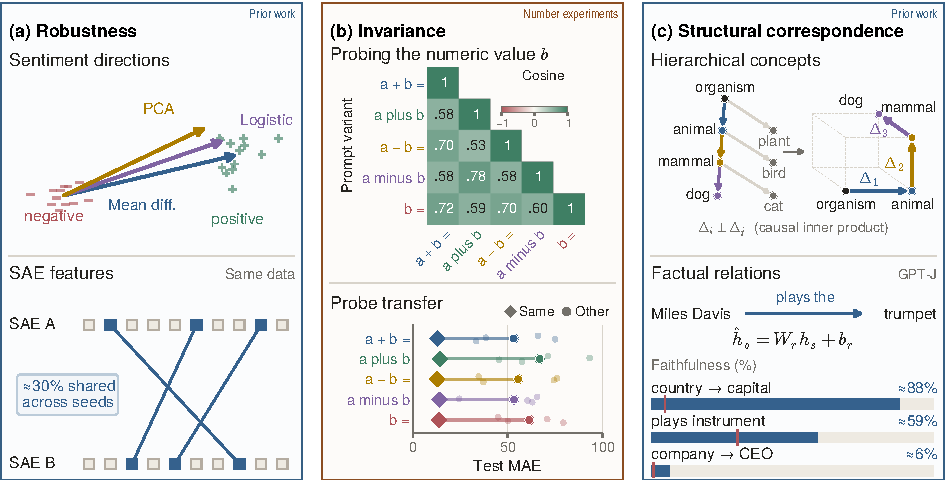
\includegraphics[width=\textwidth]{../figures/fig_robustness_invariance_structure_space_optimized.pdf}
\caption{Robustness and invariance receive mixed support, with structural correspondence observed for specific semantic relations.
The panels show agreement across estimates, transfer across prompts, and semantic relations in activation space.
(a) Sentiment directions agree across methods \citep{tigges2023linear} (top), but about 30\% of SAE features are shared across seeds \citep{paulo2026sparse} (bottom).
(b) Numerical probe directions vary across prompt variants (top), and transferred probes have large errors (bottom).
Small circles show transfer errors for individual target variants; large circles show their mean, and diamonds show within-variant error.
Summaries average six models and eleven relative layers on one fixed value-disjoint split.
(c) Orthogonal differences can encode a concept hierarchy \citep{park2025geometry} (top).
For factual relations, relation-specific linear maps predict object states $\hat h_o$ from subject states $h_s$, with varying faithfulness across relations \citep{hernandez2024linearity} (bottom).
Bars measure this faithfulness by first-token agreement with the full model; red marks show random guess.}
\label{fig:robustness-invariance-structure}
\end{figure*}
